\chapter{果蝇轮廓提取和追踪} \label{chapter:fly_contour}

果蝇轮廓提取的目标是从果蝇视频中分离出果蝇活动台、果蝇身体和果蝇翅膀,进而为提取果蝇特征做准备。其中,果蝇活动台一般为纯色背景,在不同的拍摄环境下,可能存在程度不等的噪声;果蝇身体一般为深色,和浅色的果蝇活动台差异明显,相对来说比较容易区分;果蝇翅膀呈半透明状,在视频中,果蝇翅膀区域的灰度往往介于身体和活动台之间,且翅膀的姿态往往存在较多的变化,如,果蝇可能存在振单翅、振双翅、收拢翅膀等,在不同的姿态下翅膀也表现出不同的形态。果蝇的翅膀是果蝇行为的重要特征,其中,果蝇在打架时振翅可能是一种威胁信号;而在求偶行为中,振翅也是求偶的信号。准确提取出果蝇翅膀是果蝇行为分析的基本要求。

此外,果蝇视频的拍摄环境不统一,给果蝇的身体轮廓提取带来很大的考验。现有的果蝇轮廓提取算法一般对果蝇的拍摄环境有专门的限制,比如,特定的光照条件、较高精度的拍摄设备等,给果蝇行为分析算法增加了不少限制。

本章提出一种基于背景模型的果蝇轮廓提取算法,在单高斯背景模型的基础上,对视频进行初步建模,进而在初步模型的基础上,分离果蝇活动台、果蝇身体和果蝇翅膀,通过对活动台单独建模,得到更准确的果蝇活动台模型。

\section{果蝇轮廓提取的背景模型}

果蝇身体轮廓提取的目标是从包含单独果蝇活动台的视频中,分离出多只果蝇的身体、翅膀和活动台的背景。和一般的前景物体提取不同,果蝇活动台相对比较简单,受到运动、光照等因素的影响较小;前景部分果蝇的面积和背景相比较小;前景目标在整个视频中始终存在;此外,果蝇翅膀的特殊性也对背景模型提出很高的精度要求。

%%%%%%%%%%%%%%%%%%%%%%%%%%%%%%%%%%%%%%%%%%%%%%%%%%%%%%%%%%%%
%                      果蝇活动台的初步模型
%%%%%%%%%%%%%%%%%%%%%%%%%%%%%%%%%%%%%%%%%%%%%%%%%%%%%%%%%%%%
\subsection{果蝇视频的初步背景建模}\label{sec:fly_bg_model_basic}

本章介绍一种算法,通过用单高斯背景模型和亮度畸变模型对果蝇视频进行背景建模,实现对果蝇身体和翅膀轮廓的提取。

首先,从果蝇视频中抽取$K$帧$I_{1}, I_{2}, \ldots, I_{K}$,并计算该$K$帧视频的均值$\mu$和方差$\sigma^2$,作为活动台的均值和方差;

然后,计算视频帧$I_{1}, I_{2}, \ldots, I_{K}$的亮度畸变。亮度畸变的计算公式如(\ref{eq:brightness_distortion})所示\cite{shadow_2000}:
\begin{equation}\label{eq:brightness_distortion}
\alpha(m,n) = \frac{
        \frac{I_R(m, n)\mu_R(m, n)}{\sigma_R^2(m, n)} +
        \frac{I_G(m, n)\mu_G(m, n)}{\sigma_G^2(m, n)} +
        \frac{I_B(m, n)\mu_B(m, n)}{\sigma_B^2(m, n)}
    }{
        \left[\frac{\mu_R(m, n)}{\sigma_R(m, n)}\right]^2 +
        \left[\frac{\mu_G(m, n)}{\sigma_G(m, n)}\right]^2 +
        \left[\frac{\mu_B(m, n)}{\sigma_B(m, n)}\right]^2
    },
\end{equation}
其中,$m, n$表示图像中元素的坐标,R、G、B表示色彩通道。亮度畸变可以较好的描述图像中的阴影部分,而果蝇的翅膀呈现的半透明状态和阴影在一定程度上类似。亮度畸变的引入有助于提取果蝇翅膀\cite{chexiangqian}。视频的亮度畸变$\alpha$描述了视频帧和平均值,即活动台背景$\mu$的偏离程度,其中,果蝇身体所在区域和活动台背景差异较大,亮度畸变的取值一般来说也比较小;果蝇翅膀次之,果蝇活动台部分一般最高。通过对亮度畸变进行阈值化可以大致分离出果蝇的身体、翅膀和果蝇活动台。

进一步计算视频亮度畸变的空间分布,计算$I_{1}, I_{2}, \ldots, I_{K}$的亮度畸变$\alpha_1, \alpha_2, \ldots, \alpha_{K}$的均方差,即$\textrm{RMS}(\alpha)$,并利用$\textrm{RMS}(\alpha)$对亮度畸变$\alpha$进行归一化。$\textrm{RMS}(\alpha)$的表达式如下所示:
\begin{equation} \label{eq:alpha_RMS}
\textrm{RMS}\left(\alpha(m,n)\right) =
\sqrt{\frac{\sum_{i=1}^{K} \left(\alpha_{i}(m,n)-\bar{\alpha}(m,n)\right)^2}{K}},
\end{equation}
其中,$\bar{\alpha}$表示$K$视频的亮度畸变$\alpha_1, \alpha_2, \ldots, \alpha_K$的均值,根据式(\ref{eq:brightness_distortion})的定义,易得$\bar{\alpha} = 1$。用$\textrm{RMS}(\alpha)$对$\alpha$进行归一化的原因在于,受限于拍摄条件,果蝇视频中一般存在噪声,且在视频的不同区域噪声的幅度不尽相同。

$\textrm{RMS}(\alpha)$的取值主要由两部分构成:一部分是果蝇身体和翅膀的运动,另一部分是视频拍摄过程中带来的噪声。当果蝇频繁移动时,$\textrm{RMS}(\alpha)$的取值主要由前一部分构成。使用$\textrm{RMS}(\alpha)$对$\alpha_i$进行归一化,可以降低将噪声误判为果蝇身体的可能。

归一化后的亮度畸变$\hat{\alpha}(m,n) = \alpha(m,n)/\textrm{RMS}\left(\alpha(m,n)\right)$。进一步将$\hat{\alpha}$归一化到区间$[0, 1]$,得到最终亮度畸变$\tilde{\alpha}$。果蝇的身体和翅膀可以通过对$\tilde{\alpha}$的阈值化来实现:
\begin{flalign} \label{eq:body_and_wing_model_basic}
I_{i, body} &= \left(\tilde{\alpha}_i < \tau_{body}\right), \\
I_{i, wing} &= \left(\tilde{\alpha}_i > \tau_{body} \quad \text{and} \quad \tilde{\alpha}_i < \tau_{wing}\right),
\end{flalign}
其中,$\tau_{body}$和$\tau_{wing}$通过经验设定。经验表明,$\tau_{body}$和$\tau_{wing}$对实验环境不敏感,在不同的拍摄场景和实验环境下波动很小。

此外,$\textrm{RMS}(\alpha)$还反应了果蝇的活动情况,果蝇移动频繁的区域,$\textrm{RMS}(\alpha)$较大,果蝇移动不频繁的区域,$\textrm{RMS}(\alpha)$取值较小。通过$\textrm{RMS}(\alpha)$可以得到精确果蝇活动台内径\cite{chexiangqian}。对$\textrm{RMS}(\alpha)$做阈值化处理:
\begin{equation}
I_{active} = \left( \textrm{RMS}(\alpha) > \tau_{active} \right),
\end{equation}
其中$\tau_{active}$取$\textrm{RMS}(\alpha)$的平均值即可。$I_{active}$表示了果蝇活动区域,求$I_{active}$的最小外包圆,得到果蝇活动台的精确位置。上述实现的前提是果蝇在活动台中频繁移动,且移动轨迹覆盖果蝇活动台的最外侧,上述条件很容易满足:经验表明,果蝇喜欢沿活动台的边缘追逐、爬行,利用果蝇的活动求解果蝇活动台的算法在大多数情况下都试用。

综上,果蝇活动台的均值$\mu$、方差$\sigma^2$和亮度畸变的均方差$\textrm{RMS}(\alpha)$构成了果蝇活动台轮廓提取的初步模型,记该模型为$\textrm{M}_1$。

综上,果蝇背景模型$\textrm{M}_1$的训练步骤参见算法~\ref{alg:fly_contour_model1_train}。

\begin{algorithm}
\caption{基于背景模型$\textrm{M}_1$的果蝇轮廓提取算法(训练)}
\label{alg:fly_contour_model1_train}
\begin{algorithmic}[1]
\INPUT
    \Statex 果蝇行为视频;
\OUTPUT
    \Statex 果蝇活动台背景的均值$\mu$;
    \Statex 果蝇活动台背景的方差$\sigma^{2}$;
    \Statex 果蝇活动台背景亮度畸变的均方差$\textrm{RMS}(\alpha)$;

\State 对果蝇视频进行$K$帧抽样,得到视频帧$I_{1}, I_{2}, \ldots, I_{K}$;
\State 计算视频帧$I_{1}, I_{2}, \ldots, I_{K}$的均值$\mu$和方差$\sigma^2$;
\For {$i = 1 \text{ to } K$;}
    \State 根据式(\ref{eq:brightness_distortion})计算视频帧$I_{i}$的亮度畸变$\alpha_i$;
\EndFor
\State 根据果蝇视频的亮度畸变$\alpha_1, \alpha_2, \ldots, \alpha_K$,求解亮度畸变的均方差$\textrm{RMS}(\alpha)$;
\State 输出果蝇活动台背景的均值$\mu$、果蝇活动台背景的方差$\sigma^{2}$和果蝇活动台背景亮度畸变的均方差$\textrm{RMS};(\alpha)$
\end{algorithmic}
\end{algorithm}

根据果蝇背景模型$\textrm{M}_1$进行果蝇身体轮廓提取的流程如算法~\ref{alg:fly_contour_model1_test}所示。

\begin{algorithm}
\caption{基于背景模型$\textrm{M}_1$的果蝇轮廓提取算法}
\label{alg:fly_contour_model1_test}
\begin{algorithmic}[1]
\INPUT
    \Statex 果蝇视频帧$I$;
    \Statex 果蝇活动台背景的均值$\mu$;
    \Statex 果蝇活动台背景的方差$\sigma^{2}$;
    \Statex 果蝇活动台背景亮度畸变的均方差$\textrm{RMS}(\alpha)$;
    \Statex 果蝇身体和翅膀阈值$\tau_{body}$和$\tau_{wing}$;
\OUTPUT
    \Statex 果蝇身体$I_{body}$和果蝇翅膀$I_{wing}$;

\State 根据式(\ref{eq:brightness_distortion})计算视频帧$I$的亮度畸变$\alpha$;
\State 根据式(\ref{eq:alpha_RMS})计算果蝇视频的正则化的亮度畸变$\hat{\alpha}$;
\State 将$\hat{\alpha}$归一化到区间$[0, 1]$,得到$\tilde{\alpha}$;
\State 根据$\tau_{body}$和$\tau_{wing}$对果蝇视频进行阈值化,得到果蝇身体$I_{body}$和翅膀$I_{wing}$;
\State 输出果蝇身体$I_{body}$和果蝇翅膀$I_{wing}$。
\end{algorithmic}
\end{algorithm}

背景模型$\textrm{M}_1$中,根据式(\ref{eq:body_and_wing_model_basic}) 可以得到果蝇的身体和翅膀。但是,在上面的做法中存在一个问题:我们假设$\mu$和$\sigma^2$分别表示果蝇背景的均值和方差,实际上$\mu$和$\sigma^2$表示的是果蝇视频的均值和方差,$\mu$和$\sigma^2$的计算中没有消除果蝇身体和果蝇翅膀对果蝇活动台的影响,因而存在一定的误差。下面对可能带来的误差做简单分析。

假设视频中共有2只果蝇,且2只果蝇的身体尺寸大小相同\footnote{一般来说,雌性果蝇的身体比雄性稍大。},面积均为$S_{fly}$;在整个视频时间段,果蝇投影面积不变;果蝇活动台的面积为$S_{c}$。按照背景模型$\textrm{M}_1$,果蝇的身体和翅膀被算入果蝇活动台背景,当果蝇身体和翅膀均匀的出现在果蝇活动台中时,背景模型中果蝇身体和翅膀所占的比例为:
\begin{equation}\label{eq:fly_area_ratio}
r = \frac{2S_{fly}}{S_{c}}.
\end{equation}

式(\ref{eq:fly_area_ratio})大致刻画了背景模型$\textrm{M}_1$中存在系统误差的量级。一般来说,果蝇面积相对活动台的面积很小,模型的误差也较小。但实际上,果蝇均匀的出现在容器内的假设不成立。一般来说,果蝇的活动范围往往局限于很小的区间,如活动台侧壁。在果蝇活动频繁的区域,$\textrm{M}_1$模型的果蝇活动台亮度明显偏暗。在亮度畸变的计算公式(\ref{eq:brightness_distortion})中,$I$和$\mu$是等价的,偏暗的背景和偏暗的果蝇都会使得亮度畸变值偏低,进而体现在式(\ref{eq:body_and_wing_model_basic})中,影响果蝇轮廓提取的准确性。为此,我们在本章节接下来的内容中提出一种更精确的果蝇轮廓提取模型。

%%%%%%%%%%%%%%%%%%%%%%%%%%%%%%%%%%%%%%%%%%%%%%%%%%%%%%%%%%%%
%                      果蝇活动台的精确模型
%%%%%%%%%%%%%%%%%%%%%%%%%%%%%%%%%%%%%%%%%%%%%%%%%%%%%%%%%%%%
\subsection{果蝇活动台的精确建模}\label{sec:fly_bg_model_model2}

背景模型$\textrm{M}_1$的问题主要在果蝇身体和翅膀被记入了果蝇活动台背景部分,为了解决该问题,可以首先分离果蝇活动台和果蝇身体、果蝇翅膀,具体方法用式(\ref{eq:body_and_wing_model_basic}),然后单独对果蝇活动台部分建立背景模型。下面具体介绍该算法的实现步骤。

首先,对视频帧$I_{1}, I_{2}, \ldots, I_{K}$建立单高斯背景模型模型$\textrm{M}_1$。根据式(\ref{eq:body_and_wing_model_basic})分割果蝇身体$I_{body, i}$、翅膀$I_{wing, i}$和活动台,并计算果蝇活动台的均值$\mu'$和方差$\sigma'^2$:
\begin{flalign}\label{eq:gaussian_model2}
\mu'(m, n) &= \frac{\sum_{i=1}^{K}F_i(m, n)I_i(m, n)}{\sum_{i=1}^{K}F_i(m, n)} \\
\sigma^{\prime 2}(m, n) &=
    \frac
        {\sum_{i=1}^{K}F_i(m, n)\left(I_i(m, n) - \mu'(m,n)\right)^{2}}
        {\sum_{i=1}^{K}F_i(m, n)}
\end{flalign}
其中,$F_i(m,n)$取0或1,$F_i(m,n) = 0$表示帧$I_i$在坐标$(m, n)$的像素对应果蝇身体或翅膀,$F_i(m,n) = 1$表示对应像素属于果蝇活动台。$\textrm{M}_1$模型提取的果蝇身体和翅膀并不完全准确,但对式(\ref{eq:gaussian_model2})来说,我们仅希望$\textrm{M}_1$不要将果蝇身体或翅膀判定为果蝇活动台,反之并没有严格的要求。所以在本步骤中,可以适当对式(\ref{eq:body_and_wing_model_basic})中的$\tau_{body}$和$\tau_{wing}$加以调整,使果蝇的身体和翅膀条件更加宽松。

同样的,计算视频的亮度畸变公式更新为:
\begin{equation}\label{eq:brightness_distortion_model2}
\alpha'_{m,n} = \frac{
        \frac{I_R(m, n)\mu^{\prime}_R(m, n)}{\sigma_R^{\prime 2}(m, n)} +
        \frac{I_G(m, n)\mu^{\prime}_G(m, n)}{\sigma_G^{\prime 2}(m, n)} +
        \frac{I_B(m, n)\mu^{\prime}_B(m, n)}{\sigma_B^{\prime 2}(m, n)}
    }{
        \left[\frac{\mu^{\prime}_R(m, n)}{\sigma^{\prime}_R(m, n)}\right]^2 +
        \left[\frac{\mu^{\prime}_G(m, n)}{\sigma^{\prime}_G(m, n)}\right]^2 +
        \left[\frac{\mu^{\prime}_B(m, n)}{\sigma^{\prime}_B(m, n)}\right]^2
    }.
\end{equation}

亮度畸变$\alpha_1, \alpha_2, \ldots, \alpha_K$的均方差$\textrm{RMS}(\alpha')$的计算公式为:
\begin{equation}
\textrm{RMS}\left(\alpha'(m, n)\right) = \sqrt{
    \frac{
        \sum_{i=1}^{K}F_i(m,n)\left(\alpha'_{i}(m, n)-\bar{\alpha'}(m, n)\right)^2}
        {\sum_{i=1}^{K}F_i(m,n)}
}.
\end{equation}

果蝇活动台的均值$\mu'$和方差$\sigma'^2$和亮度畸变的均方差$\textrm{RMS}(\alpha')$构成新的精确模型,记为$\textrm{M}_2$。利用$\textrm{M}_2$计算果蝇的身体和翅膀的流程和第\ref{sec:fly_bg_model_basic}章的过程类似,首先,利用$\textrm{RMS}(\alpha')$对亮度畸变$\alpha'$的归一化:
\begin{equation}
\hat{\alpha}'(m, n) = \frac{\alpha'(m, n)}{\textrm{RMS}\left(\alpha'(m, n)\right)},
\end{equation}

进而将$\hat{\alpha}'$归一化到区间$[0, 1]$,得到$\tilde{\alpha}'$。通过阈值化$\tilde{\alpha}'$,完成果蝇身体和翅膀的轮廓提取。对视频帧$I_i$,果蝇身体$I_{i, body}$和果蝇翅膀$I_{i,wing}$的计算表达式为:
\begin{flalign}\label{eq:fly_contour_model2}
I_{i, body} &= \left(\tilde{\alpha}'_i < \tau_{body}\right), \\
I_{i, wing} &= \left(\tilde{\alpha}'_i > \tau_{body} \quad \text{and} \quad \tilde{\alpha}'_i < \tau_{wing}\right).
\end{flalign}

因为剔除了果蝇身体和翅膀对背景的影响,因而式(\ref{eq:fly_contour_model2})中得到的果蝇身体$I_{i, body}$和果蝇翅膀$I_{i,wing}$更加精确。

背景模型$\textrm{M}_2$的完整求解流程可以用算法~\ref{alg:fly_contour_model2_train}来描述:

\begin{algorithm}
\caption{果蝇精确}
\label{alg:fly_contour_model2_train}
\begin{algorithmic}[1]
\INPUT
    \Statex 果蝇行为视频;
    \Statex 果蝇活动台背景模型$\textrm{M}_1$;
\OUTPUT
    \Statex 果蝇活动台均值$\mu'$;
    \Statex 果蝇活动台方差$\sigma^{\prime 2}$;
    \Statex 果蝇活动台亮度畸变的均方差$\textrm{RMS}(\alpha')$;
\State 对果蝇视频进行$K$帧采样,得到视频帧$I_{1}, I_{2}, \ldots, I_{K}$;
\For {$i = 1 \text{ to } K$; }
    \State 利用$\textrm{M}_1$模型,计算视频帧$I_i$中的果蝇身体$I_{i, body}$和翅膀$I_{i, wing}$;
\EndFor
\State 根据式(\ref{eq:gaussian_model2}),计算更新的果蝇活动台均值$\mu'$和方差$\sigma^{\prime 2}$
\For {$i = 1 \text{ to } K$; }
    \State 求视频帧$I_{i}$的亮度畸变$\alpha'_{i}$;
\EndFor
\State 计算果蝇行为视频中活动台的亮度畸变$\alpha'_{1}, \alpha'_{2}, \ldots, \alpha'_{K}$的均方差$\textrm{RMS}(\alpha')$;
\State 输出果蝇活动台均值$\mu'$、果蝇活动台方差$\sigma^{\prime 2}$、果蝇活动台亮度畸变的均方差$\textrm{RMS}(\alpha')$。
\end{algorithmic}
\end{algorithm}

根据背景模型$\textrm{M}_2$求果蝇身体和翅膀的流程和算法~\ref{alg:fly_contour_model1_test}类似,在此不做详细的介绍。

\subsection{果蝇身体轮廓的自适应}

最后,本章简要介绍使用果蝇的身体尺寸对果蝇身体进行自适应的算法。作为对模型$\textrm{M}_2$的必要补充,自适应的引入可以提高算法的鲁棒性。

首先,对视频进行$K$帧抽样,并使用第\ref{sec:fly_locate}章中果蝇身体尺寸求解算法,计算每一帧$I_i$中果蝇身体的尺寸$(a_i, b_i)$。然后,求解果蝇身体尺寸$(a_1, b_1),(a_2, b_2), \ldots, (a_K, b_K)$的中位数,得到果蝇身体的最终尺寸$(a, b)$。需要注意的是,为了得到更加准确的果蝇身体尺寸,应该仅计算果蝇连通域数目和果蝇数目相等的帧。

在假设果蝇身体为椭圆形的情况下,计算果蝇身体约等于$S=\pi ab$。根据背景模型$\textrm{M}_2$,得到果蝇身体部位$I_{body}$和翅膀部位$I_{wing}$,分别求身体部位的实际面积$S_{body}$和翅膀部位的实际面积$S_{wing}$,并分别引入变量$r_{body}$和$r_{wing}$:
\begin{flalign}\label{eq:fly_contour_ratio_adptive}
r_{body} &= \frac{S_{body}}{2S}, \\
r_{wing} &= \frac{S_{wing}}{2S}.
\end{flalign}

对于视频中包含果蝇数目不为2的情况,需要对(\ref{eq:fly_contour_ratio_adptive})进行相应的调整。

分别对果蝇翅膀和果蝇身体进行自适应,流程如下:如果$r_{wing} < r_{wing,lower}$,说明翅膀的面积偏小,应该增加$\tau_{wing}$的值以增加检测到的果蝇翅膀面积。反之,如果$r_{wing} > r_{wing, upper}$,则说明果蝇的翅膀面积偏大, 应该减小$\tau_{wing}$以降低检测到的果蝇翅膀的面积。$\tau_{wing}$的调整可以采用增加或者减少一个固定的值$\Delta_{wing}$来实现,即$\tau^{\{i+1\}}_{wing} = \tau^{\{i\}}_{wing} \pm \Delta_{wing}$,其中$i$表示自适应的次数,$\tau^{\{i\}}_{wing}$表示第$i$轮自适应的翅膀阈值参数。根据调整后的翅膀阈值$\tau^{\{i+1\}}_{wing}$重新计算果蝇翅膀$I_{wing}$和对应的面积$S_{wing}$,进而重新计算$r_{wing}$。对上述步骤进行若干次,即可实现翅膀的自适应。

对果蝇身体部位的自适应过程与之类似。在果蝇翅膀自适应完成后,进行果蝇身体的自适应。当$r_{body} < r_{body, lower}$时,说明果蝇身体的面积偏小,需要减小$\tau_{body}$来增加检测到的果蝇身体的面积;反之,如果$r_{body} > r_{body, upper}$,说明果蝇身体的面积偏大,需要增加$\tau_{body}$的值。对上述步骤进行若干次调整,即可完成身体部分的自适应。

果蝇身体和翅膀的自适应算法进一步提高了果蝇轮廓提取算法的鲁棒性,使得算法对不同拍摄环境下的果蝇行为视频都能取得较好的结果。

%%%%%%%%%%%%%%%%%%%%%%%%%%%%%%%%%%%%%%%%%%%%%%%%%%%%%%%%%%%%
%                      果蝇的定位和追踪
%%%%%%%%%%%%%%%%%%%%%%%%%%%%%%%%%%%%%%%%%%%%%%%%%%%%%%%%%%%%
\section{果蝇的定位和追踪} \label{sec:fly_discrimination_and_track}

\subsection{果蝇身体的定位}\label{sec:fly_locate}

得到果蝇的身体和翅膀的区域后,需要进一步的计算每只果蝇的位置。令$I_{fly}$表示果蝇身体和翅膀所在区域,求$I_{fly}$的连通域。当果蝇活动台中有2只果蝇时,理论上应该出现2个连通区域,且每个连通区域和单只果蝇分别对应。但实际上,考虑到果蝇行为视频中,果蝇在部分情况下存在身体接触、甚至求偶时果蝇完全抱在一起,使得$I_{fly}$中仅存在一个连通区域;在部分情况下,果蝇侧立在活动台的侧壁,果蝇翅膀遮盖住果蝇部分身体,比如果蝇腹部,使得果蝇腹部的灰度明显比正常的果蝇身体亮,在根据式(\ref{eq:body_and_wing_model_basic})求解果蝇身体时出现果蝇身体在腹部出现明显的断裂,导致$I_{fly}$中的连通区域数目超过果蝇的数目。此外,果蝇视频中可能存在光线的亮度、噪声等都可能对连通域的数目带来影响,造成连通域数目和果蝇数目不一致的问题。

在果蝇连通域数目$k$和果蝇数目$K$一致时,我们可以认为每个连通域和果蝇身体相对应。果蝇的身体轮廓可以被建模成椭圆\cite{chexiangqian}。但是,求解连通域的最小外包椭圆相对比较困难,我们可以用最小外包矩形代替。最小外包矩形可以用参数$\{(x, y), (A, B), \theta\}$来表示,其中$(x, y)$表示外包矩形中心的坐标,$(A, B)$表示外包矩形的长和宽,$\theta$表示外包矩形长边的方向。在椭圆形假设下,果蝇身体的长轴和短轴分别为$(a, b) = (A/2, B/2)$。求解最小外包矩形的计算复杂度为线性复杂度,不超过最小外包矩形的面积\cite{Freeman:1975:DME:360881.360919}。通过求解最小外包矩形的参数,可以得到果蝇身体的位置、大小和方向。

对于连通域数目和果蝇身体数目不一致的情况,应分两种情况:连通域的数目$k$大于果蝇数目$K$;或连通域的数目$k$小于果蝇数目$K$。下面分别对上述情况加以考虑。

$k>K$时,一般是因为果蝇的身体某部分可能出现了不连通的情况,可以通过对果蝇身体$I_{fly}$的坐标进行聚类,将身体所在像素的坐标聚类为果蝇的数目,聚类结果的每一类别对应一只果蝇。和上述求解果蝇身体位置、大小的方式一样,通过求解最小外包矩形求解果蝇身体参数$\{(x, y), (A, B), \theta\}$。根据问题的特点,选择使用采用Single-Linkage的层次聚类(Hierarchical Clustering)算法\cite{rokach2005clustering},像素点的距离采用4-近邻距离。

$k<K$时,使用细胞分割算法${}^{\cite{cell_seg_2010}}$。连通域数目小于果蝇数目时,一般是因为果蝇之间存在身体接触。细胞分割算法专门用于分离接触的目标,当物体有小面积接触时效果较好,在大面积重合时算法的性能不尽人意,主要是因为细胞分割算法只能把重叠区域分配给其中1个物体,因而有重叠的目标都比实际要小。该算法的主要思路也是对坐标进行聚类,但是在聚类时考虑到了每个像素的权重不同,位于连通域边缘的像素具有较小的权重,而位于连通域中心的像素具有较大的权重。聚类一般采用混合高斯模型实现,距离尺度使用欧氏距离。通过\cite{cell_seg_2010}中的算法,将果蝇身体划分成不同的连通域,并通过求解最小外包矩形求解果蝇身体的参数$\{(x, y), (A, B), \theta\}$。上述算法在处理求偶时完全重叠的果蝇时会出现问题,在今后的研究中可以综合考虑果蝇的姿态等,以减少上述算法对果蝇身体分割带来的影响。

通过上述步骤,求出分离的果蝇,并求出每只果蝇的基本身体参数$\{(x, y), (A, B), \theta\}$。

\subsection{果蝇的追踪}\label{sec:fly_track}

根据第\ref{sec:fly_locate}章中的算法,可以确定每一帧中果蝇身体的位置$(x, y)$和身体朝向$\theta$。但是,在不同的帧间,我们需要确定不同果蝇的对应关系,即编号问题。此外,根据果蝇轮廓的外包矩形只能判断身体的朝向,并不能直接确定果蝇头部的方向,还需要进一步判断果蝇头部的朝向。

首先,考虑果蝇之间的对应关系。果蝇的身体结构比较简单,不同个体之间的差异性不大,在实验环境下,很难通过视频的图形学特征判断果蝇的编号。为此,可以根据运动信息来判定:
% \DeclareMathOperator*{\argmin}{arg\,min}
\begin{equation}\label{eq:fly_dicrimination}
\underset{n_{1},n_2, \ldots, n_K}{arg\,min}
\sum_{i=1}^K\|\vec{P}_{c, n_i} - \vec{P}_{c, i}\|_2^2
\end{equation}

其中,$\vec{P}_{c, i}$表示第$i$只果蝇身体重心的位置,$n_i$表示下一帧中果蝇$i$的新编号,$n_i$的取值是$\left\{1,2,\ldots,K\right\}$的一个排列组合。通过最小化式(\ref{eq:fly_dicrimination})中的目标函数,基本可以保证果蝇序号不发生交换。

外包矩形给出了果蝇身体的参数$\left\{(x, y), (a, b), \theta\right\}$,其中$\theta$只给出了果蝇身体的朝向,果蝇的头部方向可能是$\theta$或$\theta+\pi$。为了确定果蝇头部的方向,可以考虑以下几种特征:
\begin{enumerate}
\item 根据果蝇的形态特征进行判断;
\item 根据果蝇的运动特征进行判断;
\item 根据果蝇上一帧的结果进行判断;
\end{enumerate}

首先,根据果蝇的形态特征进行判断。考虑到果蝇的身体形态特征,从图形学的角度判断果蝇的头部和尾部的方法不太多,目前比较常用的是根据头部和尾部的灰度差异判断。果蝇的翅膀一般收缩在尾部,因而尾部的亮度会比头部稍微高一些。图像亮度较低的是头部,图像亮度较高的是尾部。此外,还有根据果蝇头部和尾部轮廓的曲率判断果蝇头部和尾部的方式。

其次,根据果蝇在帧间的运动特征进行判断。正常情况下,果蝇会选择向前移动。计算每两帧之间果蝇的运动方向,其头部朝向在大多数情况下和果蝇的运动方向应该是一致的,尾部朝向和运动方向相反。但是考虑到果蝇在部分情况下可能会静止,或者存在较小的后退,比如,在打架行为中,果蝇为了蓄力往往会有一个后挫动作。通过运动方向来判断果蝇的头部和尾部存在一定的问题。

最后,可以根据果蝇的上一帧结果进行判断。参考式(\ref{eq:fly_dicrimination})中的方案,通过最小化果蝇头部和尾部在帧间移动距离的平方和,完成果蝇头部和尾部的识别。对于第$i$帧中果蝇$k$,首先,求出该果蝇可能的头部位置和尾部位置$\vec{P}_{0}$和$\vec{P}_{1}$,
\begin{equation}\label{eq:fly_head_tail_dist}
\underset{i_0, i_1}{arg\,min} \left\|\vec{P}_{i_0} - \vec{P}_{h}\right\|_2^2 + \left\|\vec{P}_{i_1} - \vec{P}_{t}\right\|_2^2.
\end{equation}
其中,$\vec{P}_{h}$和$\vec{P}_{t}$分别表示第$i-1$帧中果蝇$k$的头部和尾部的位置,$i_0$、$i_1$是$\left\{0, 1\right\}$的一个排列组合。通过最小化头部和尾部的移动距离的平方和,保证果蝇头部和尾部移动的连续性,基本可以保证在正常移动情况下果蝇头部和尾部在视频中的一致性。

最后,本章综合采用果蝇的移动方向和上一阵果蝇的位置进行果蝇头部和尾部的判断。如果果蝇在前后帧的移动距离大于某阈值时,利用果蝇的移动方向确定果蝇的头部和尾部;否则,利用上一帧的果蝇头部和尾部的位置信息确定当前帧下果蝇的头部和尾部。


%%%%%%%%%%%%%%%%%%%%%%%%%%%%%%%%%%%%%%%%%%%%%%%%%%%%%%%%%%%%
%                      果蝇轮廓提取的结果和分析
%%%%%%%%%%%%%%%%%%%%%%%%%%%%%%%%%%%%%%%%%%%%%%%%%%%%%%%%%%%%
\section{果蝇轮廓提取的结果和分析}\label{sec:chap4_experiments}

本文对不同环境下拍摄的果蝇视频进行果蝇身体检测和追踪。如图~\ref{fig:bg_model_origin}所示,来自4组不同拍摄环境下的视频,从左到右依次记为视频(a)、(b)、(c)、(d),每段视频长度约为10分钟,视频的大小约为200$\times$200,清晰度和分辨率各不相同,亮度上也存在较大的差异。此外,视频中还存在相当的噪声,从视频帧(a)中可以看出,果蝇活动台的中心有浅黄色的果蝇食物,活动台的侧壁存在明暗不同的反光。在视频(b)、(c)和(d)中也存在程度不同的上述情况。除视频拍摄环境、视频质量外,(a)、(b)、(c)、(d)视频中包含不同的果蝇尺度和姿态,图~\ref{fig:bg_model_origin}中包括了果蝇侧立、正趴、追尾以及求偶等不同的形态,在不同的形态中,果蝇的翅膀也呈现出不同的形态特征,如,(a)中翅膀收在尾部,(b)中右下角的果蝇翅膀展开,(c)、(d)中果蝇翅膀因侧立等原因呈现出细、尖的特点。

针对上述不同视频,分别用大律法、背景模型$\textrm{M}_1$和背景模型$\textrm{M}_2$进行果蝇轮廓的提取。其中,背景模型$\textrm{M}_1$和背景模型$\textrm{M}_1$的参数阈值$\tau_{wing} = 0.63, \tau_{body} = 0.42$,并对阈值$\tau_{wing}$和$\tau_{body}$进行自适应,自适应的步长为0.01,最多自适应步数10次。

\begin{figure}
\centering
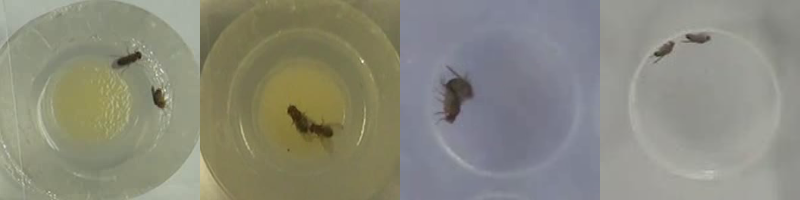
\includegraphics[width=0.9\textwidth]{bg_model_origin}
\caption{果蝇视频示例}
\label{fig:bg_model_origin}
\end{figure}

大律法提取果蝇轮廓的结果如图~\ref{fig:bg_model_ostu}所示,其中,白色、黑色分别表示果蝇身体和活动台背景。图~\ref{fig:bg_model_ostu}表明,大律法提取果蝇轮廓的结果很差,视频(a)、(d)中果蝇轮廓和活动台背景混杂在一起,无法分开。这是因为视频(a)、(d)的拍摄环境比较简单,果蝇活动台的颜色并不均一,其暗色部分和果蝇翅膀效果比较接近,仅仅依靠像素灰度无法有效的提取果蝇的身体和翅膀。

\begin{figure}
\centering
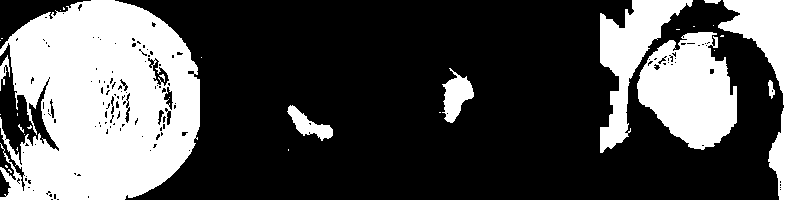
\includegraphics[width=0.9\textwidth]{bg_model_ostu}
\caption{大律法求果蝇轮廓结果}
\label{fig:bg_model_ostu}
\end{figure}

下面详细讨论背景模型$\textrm{M}_1$和背景模型$\textrm{M}_2$。以视频(d)为例,计算视频模型中的背景图像,并计算和原始的视频帧的差,其中视频图像如图~\ref{fig:frame}所示,模型$\textrm{M}_1$和$\textrm{M}_2$求解的活动台背景如图~\ref{fig:frame_mean_model1}和图~\ref{fig:frame_mean_model2}所示。

\begin{figure}
\centering
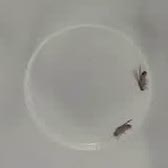
\includegraphics[width=0.25\textwidth]{frame}
\caption{原始果蝇视频}\label{fig:frame}
\end{figure}

\begin{figure}
\centering
\subcaptionbox{模型$\textrm{M}_1$的背景\label{fig:frame_mean}} {
    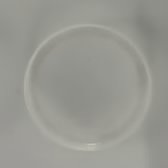
\includegraphics[width=0.25\textwidth]{frame_mean}
}
\hspace{10pt}
\subcaptionbox{背景与视频帧的差\label{fig:frame_delta}} {
    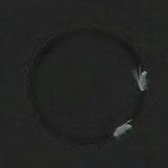
\includegraphics[width=0.25\textwidth]{frame_delta}
}
\caption{背景模型$\textrm{M}_1$的果蝇活动台模型}
\label{fig:frame_mean_model1}
\end{figure}

\begin{figure}
\centering
\subcaptionbox{模型$\textrm{M}_2$的背景\label{fig:bg_mean}} {
    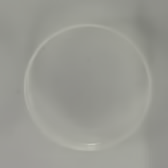
\includegraphics[width=0.25\textwidth]{bg_mean}
}
\hspace{10pt}
\subcaptionbox{背景与视频帧的差\label{fig:bg_delta}} {
    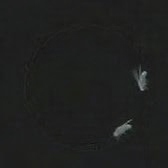
\includegraphics[width=0.25\textwidth]{bg_delta}
}
\caption{背景模型$\textrm{M}_2$下的果蝇活动台模型}
\label{fig:frame_mean_model2}
\end{figure}

图~\ref{fig:frame_mean_model1}和图~\ref{fig:frame_mean_model2}中,左侧是对应背景模型求得的活动台背景,右侧是活动台背景和原始果蝇视频帧的差。考虑到活动台背景和原始果蝇视频帧的差值中存在负值,在图~\ref{fig:frame_mean_model1}和图~\ref{fig:frame_mean_model2}中对像素值加上某个常量,使之最小值为0。对比图~\ref{fig:frame_mean_model1}和图~\ref{fig:frame_mean_model2}的背景,背景模型$\textrm{M}_1$求得的活动台在边缘区域明显比背景模型$\textrm{M}_2$要暗,这是一个因为果蝇习惯沿果蝇互动台侧壁移动。对比差值更能清楚的反映出该问题,在~\ref{fig:frame_delta}的边缘明显存在偏暗的圈,而在~\ref{fig:bg_delta}中,除果蝇身体所在区域外,其余区域基本为黑色,即果蝇活动台的背景部分被很好的剔除掉。

下面看视频帧的亮度畸变。同样对图~\ref{fig:frame}中的图像,分别用背景模型$\textrm{M}_1$和背景模型$\textrm{M}_2$求亮度畸变,结果如图~\ref{fig:model_alpha}所示。视频的亮度畸变的取值一般在$[0, 2]$之间,为了便于表示,我们把亮度畸变归一化到区间$[0, 255]$。在图~\ref{fig:model_alpha}中,果蝇身体所在的区域最暗,其次是果蝇翅膀,最后是果蝇活动台。只需要对亮度畸变进行阈值化即可得到最终的果蝇身体和果蝇翅膀。对比~\ref{fig:frame_alpha}和~\ref{fig:bg_alpha},很容易看出背景模型$\textrm{M}_2$比背景模型$\textrm{M}_1$的改进。在~\ref{fig:bg_alpha}中,果蝇活动台区域的取值更加一致,且和果蝇身体、翅膀的取值相差较大,因而采用阈值化可以得到更准确的果蝇身体和翅膀。

\begin{figure}
\centering
\subcaptionbox{模型$\textrm{M}_1$下的亮度畸变$\alpha$\label{fig:frame_alpha}} {
    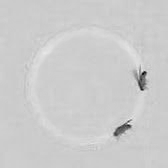
\includegraphics[width=0.25\textwidth]{frame_alpha}
}
\hspace{10pt}
\subcaptionbox{模型$\textrm{M}_2$下的亮度畸变$\alpha'$\label{fig:bg_alpha}} {
    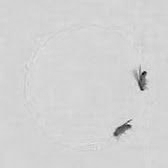
\includegraphics[width=0.25\textwidth]{bg_alpha}
}
\caption{背景模型的亮度畸变}
\label{fig:model_alpha}
\end{figure}

利用背景模型$\textrm{M}_1$和背景模型$\textrm{M}_2$提取果蝇轮廓的结果参见图~\ref{fig:bg_model_result_1}、 图~\ref{fig:bg_model_result_2}。图中,黑色、白色、灰色分别表示果蝇活动台、果蝇身体和果蝇翅膀。图~\ref{fig:bg_model_result_2}中,对于来自4个视频的帧,本文提出的背景模型都能准确的提取出果蝇的轮廓,比如,视频(b)中正趴在容器底部的果蝇张开的翅膀,以及视频(d)中趴在容器壁上侧立的果蝇的翅膀尖,均有良好的表现。同样的,图~\ref{fig:bg_model_result_1}也能找到视频中的果蝇身体和翅膀,但与此同时,该模型也会将大量的果蝇活动台判定为果蝇翅膀。这也说明对活动台单独建模的必要性。

\begin{figure}[htb]
\centering
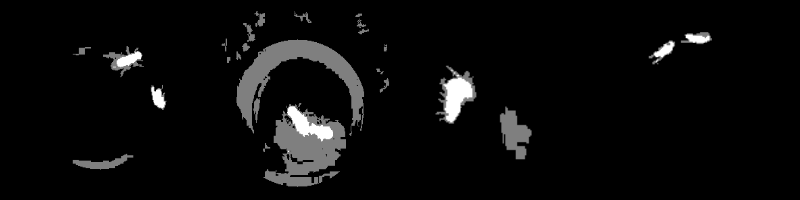
\includegraphics[width=0.9\textwidth]{bg_model_result_1}
\caption{背景模型$\textrm{M}_1$求果蝇轮廓结果}
\label{fig:bg_model_result_1}
\end{figure}

\begin{figure}[thb]
\centering
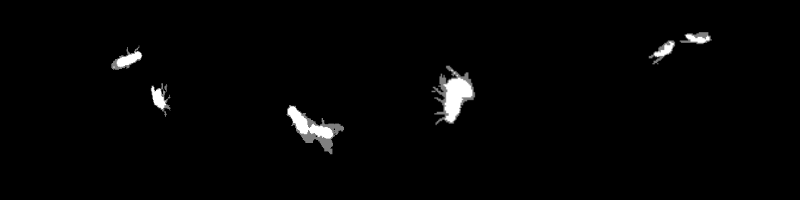
\includegraphics[width=0.9\textwidth]{bg_model_result_2}
\caption{背景模型$\textrm{M}_2$求果蝇轮廓结果}
\label{fig:bg_model_result_2}
\end{figure}

\section{小结}
针对果蝇轮廓提取的问题,本章提出了一种基于背景模型的算法。该算法先通过对果蝇视频进行初步建模,大致分割出果蝇的身体、翅膀和活动台后,进一步对活动台单独建模,得到更加准确的背景模型,进而实现果蝇身体轮廓的准确提取。仿真结果表明,本文提出的算法可以适应不同拍摄环境,具有较好的鲁棒性。

